\documentclass{acmsiggraph}
\usepackage[scaled=.92]{helvet}
\usepackage{times}

\usepackage{rotating}
\newcommand{\rotxc}[1]{\begin{sideways}#1\end{sideways}}
\newcommand{\invert}[1]{\rotxc{\rotxc{#1}}}
\usepackage{graphicx}

%% use this for zero \parindent and non-zero \parskip, intelligently.

\usepackage{parskip}
\usepackage{footnote}
\usepackage[breaklinks,hidelinks]{hyperref}

\renewcommand{\thefootnote}{\fnsymbol{footnote}}

\usepackage[labelfont=bf,textfont=it]{caption}
\usepackage{amsmath, amsthm, amssymb}

\newtheorem{thm}{Theorem}[section]
\newtheorem{cor}[thm]{Corollary}
\newtheorem{lem}[thm]{Lemma}

\theoremstyle{remark}
\newtheorem{rem}[thm]{Remark}

\theoremstyle{definition}
\newtheorem{defn}[thm]{Definition}

%Hacky pseudo-code:
\newcommand{\cF}[1]{{\tt #1}}
\newcommand{\cTAB}{\phantom{----}}
\newcommand{\cIF}{{\bf if}}
\newcommand{\cRET}{{\bf return}}
\newcommand{\cWHILE}{{\bf while}}
\newcommand{\cFOR}{{\bf for}}

\newcommand{\defbreak}{\vspace{1em}}
\title{The {\em fluint8} Software Integer Library}

\author{Jim McCann\thanks{e-mail: ix@tchow.com}\\
  TCHOW llc
  \and
  Tom Murphy VII\thanks{\protect \rotatebox[origin=c]{180}{e}-mail: tom7@tom7.org}\\
  tom7.org foundation}

\teaser{
\centering
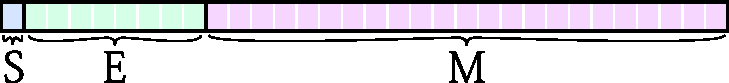
\includegraphics[width=3in]{ieee754-binary32.pdf} \huge $= -1^{S}\cdot 2^{E-127-23} \cdot (2^{23} + M)$
\caption{\label{fig-binary32}
Our library performs unsigned integer operations using only arithmetic operations on IEEE754 floating point numbers stored in binary32 format (pictured).
}}

%\keywords{anger, invective, morality}
\begin{document}

\maketitle

\begin{abstract}
We present {\em fluint8}, a library for performing integer math, including basic arithmetic and bitwise logical operations, using only basic floating point operations.
\end{abstract}
\setcounter{footnote}{2}

%D.2.3 = 0xD23 = 0x45523000 (floating point)
%         exponent:45
%0x305245
\begin{CRcatlist}
\CRcat{$(1.10100100011)_{2}\times{}2^{11}$}{Software}{Software Engineering}{\small Coding Tools and Techniques}
\end{CRcatlist}

\section{Introduction}
There are a surfeit of libraries that exist to perform floating point operations on processors that only support integer math.
This is unsurprising, as many such processors exist -- from ancient 286's to modern embedded microcontrollers.
These libraries use many integer instructions to emulate the action of a floating point unit, providing correct and useful (if slow) results.

We present a small header-only C library to emulate integer operations -- specifically 8-bit unsigned integer operations -- using standard IEEE 754 single-precision (binary32) floating point math.
Our presented operations have been designed to be succinct but also pleasantly puzzling.

As far as we are aware, no processor exists for which this library would be required.
However, perhaps you should consider that a challenge.

\section{Floating Point}
An IEEE 754 single-precision floating point number (binary32 format) is stored as a sign bit, a 8-bit exponent, and a 23-bit mantissa (Figure~\ref{fig-binary32}).
Except for special cases, the number represented by a floating point number with sign $S$, exponent $E$, and mantissa $M$ is
\footnote{or at least this is what wikipedia says, so I'm going with that, and it seems to work out.}:
\begin{displaymath}
-1^{S}\cdot (1.M)_2 \cdot 2^{E-127}
\end{displaymath}

Particularly, notice that the leading ``1'' in the fraction is implicit in the representation (it is implied by a non-zero exponent\footnote{An all-zero exponent is used for special numbers like zero, but we're not going to go into that. Wait, we just did.}).

This means that the range of integers that can be represented (without loss of precision) is
\begin{displaymath}
[-2^{24},2^{24}] = [-16777216, 16777216]
\end{displaymath}
which, conveniently, is far more than the $[0,255]$ range needed for storing 8-bit unsigned integers.

When floating point operations result in numbers that cannot be accurately represented, the results are rounded according to the current rounding mode.
The default rounding mode assumed in this paper is {\em roundTiesToEven}.
I would say that it does what you expect, but floating point numbers seldom manage that feat.
Regardless, this rounding mode means that whenever a value is exactly halfway between two representable numbers, the number with a least-significant-bit of 0 is picked.

Rounding and precision loss leads to this fun fact:
\begin{center} \tt
16777216.0f + 1.0f - 1.0f == 16777215.0f\\
16777216.0f - 1.0f + 1.0f == 16777216.0f
\end{center}
(Hot take: floating-point operations are non-commutative.)

\section{The {\em fluint8} Library}
The fluint8 library provides all of the mathematical and logical operations one expects on 8-bit integers, using only floating point addition, subtraction, multiplication, and division --
other than a loop with fixed bounds which could be unrolled by the compiler, no conditionals or function calls are required.

Full source code for the library (and this paper) are available at \url{https://github.com/ixchow/fluint8}.

In this section we go through the library operation by operation, explaining how each function works.

\subsection{Storage Format}
Our library represents unsigned 8-bit integers as their equivalent floating point values.
In other words, the value {\tt uint\_t(127)} is represented as {\tt 127.0f}.
This straightforward equivalence is convenient when writing basic mathematical functions.

In order to support, e.g., reading data from files, our library includes functions that convert between floating point numbers and bit-patterns of their equivalent 8-bit unsigned representation.

{\tt
void fu8\_to\_bits(float a, void *out) \{ \\
$\phantom{XX}$a += 8388608.0f; \\
$\phantom{XX}$memcpy(out, \&a, (size\_t)(1.0f)); \\
\}
}

The function {\tt fu8\_to\_bits} adds a large enough number to {\tt a} that its mantissa's least-significant bit now represents 1.
Essentially, the code is shoving the integer information stored in {\tt a} to the least-significant-byte of the representation, and then copying\footnote{
The astute reader will notice that we've taken care to avoid using an integer constant as a parameter to {\tt memcpy}.
Presumably on processors without integer support {\tt size\_t} must be a floating-point type.
And, yes, we promised above not to use function calls, but it's hard to copy a byte without integer types.
} it out to the destination.

The same trick works when setting a floating point number from an integer bit pattern:

{\tt
float fu8\_from\_bits(void const *from) \{ \\
$\phantom{XX}$float a = 8388608.0f; \\
$\phantom{XX}$memcpy(\&a, from, (size\_t)(1.0f)); \\
$\phantom{XX}$return a - 8388608.0f; \\
\}
}


\begin{figure}[tb!]
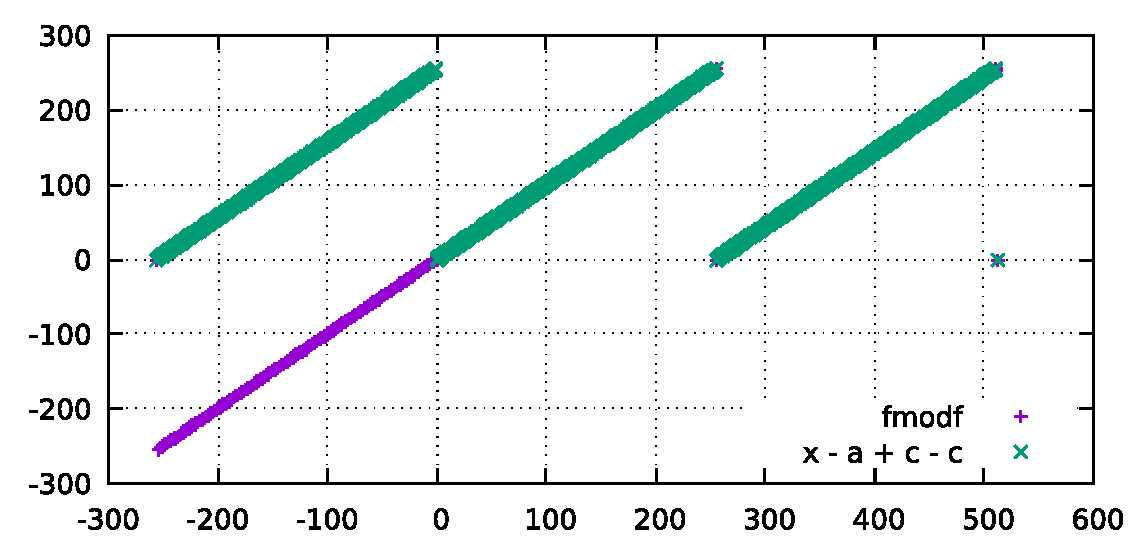
\includegraphics[width=\columnwidth]{fmodf.pdf}
\caption{\label{fig-mod-graph} Comparing {\tt fmodf(x, 256.0f)} to the expression {\tt x - 127.5f + 3221225472.0f - 3221225472.0f} over the range {\tt [-256.0f, 512.0f]}.
Notice that the expression is positive for negative numbers, making it more useful for simulating integer rollover.
{\small Plot created using gnuplot.}}
\end{figure}


\begin{figure}[tb!]
\begin{center}
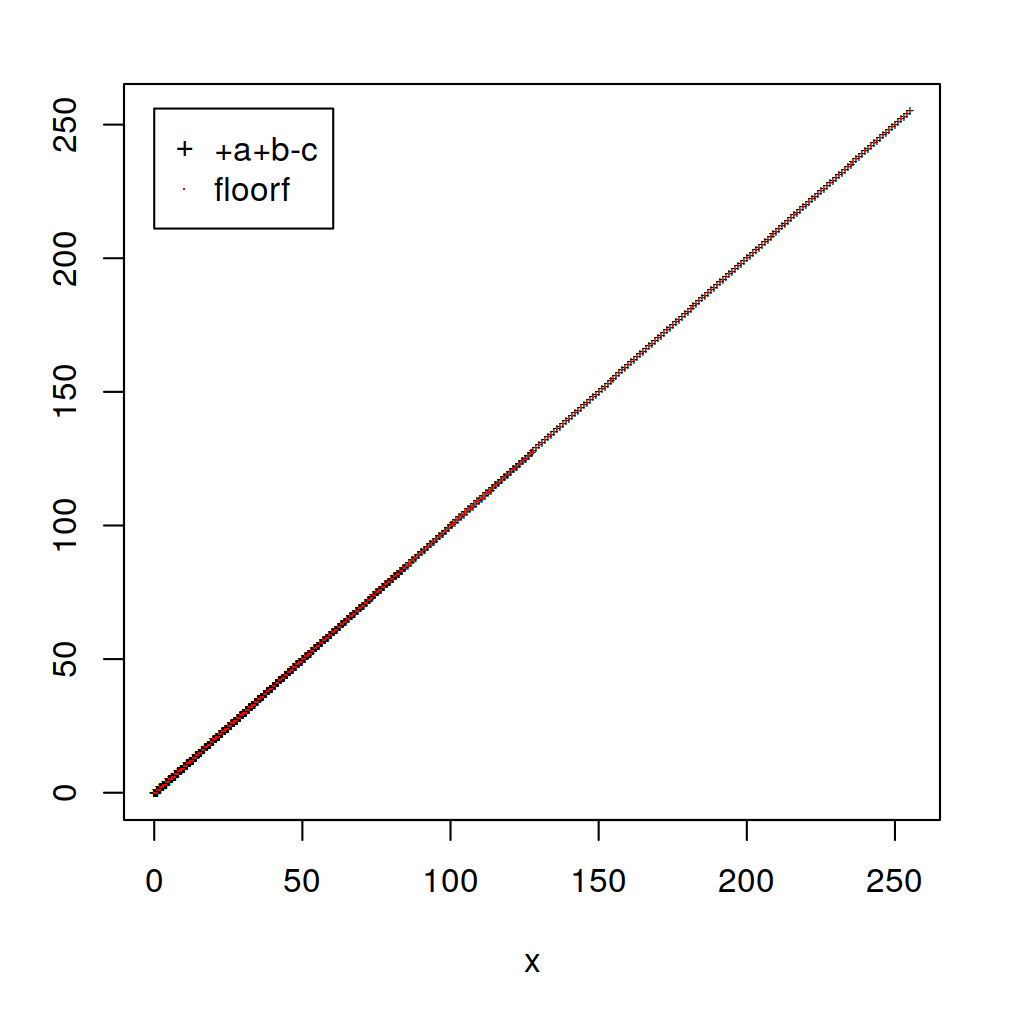
\includegraphics[width=0.49\columnwidth]{floor256.png}
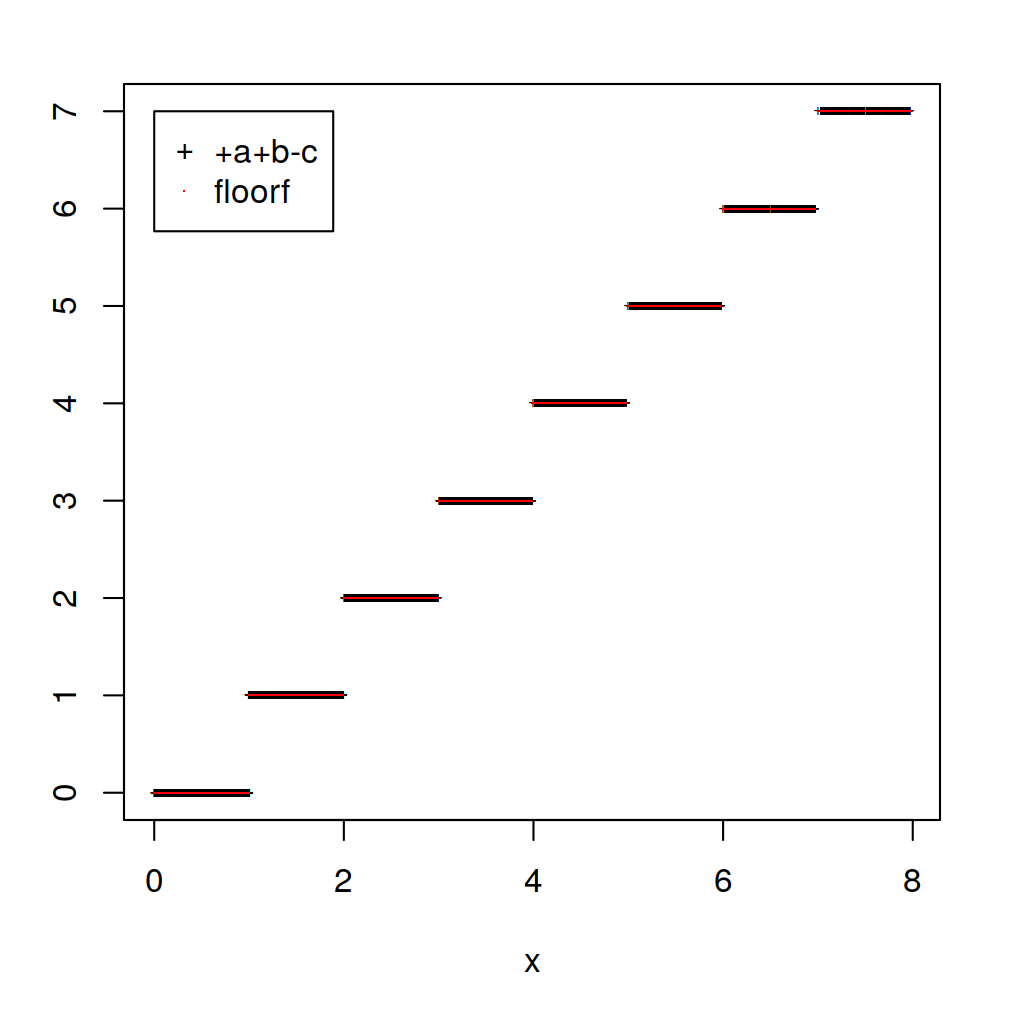
\includegraphics[width=0.49\columnwidth]{floor8.png}
\end{center}
\caption{\label{fig-floor-graph} Comparing {\tt floorf(x)} to the expression {\tt x + 0.50390625f + 8388608.0f - 8388609.0f} over the all quotients {\tt [0.0f, 255.0f] / [1.0f, 255.0f]}.
The functions match at all plotted points.
{\small Plot created using R.}}
\end{figure}


% http://en.cppreference.com/w/cpp/language/operator_arithmetic
\subsection{Arithmetic Functions}
Our library implements {\tt +}, {\tt -}, {\tt *}, {\tt /}, {\tt +}, and {\tt -} by treating floating point numbers as real numbers; an approach that often works, but requires some post-processing to deal with roll-over:

{\tt
float fu8\_add(float a, float b) \{ \\
$\phantom{XX}$float x = a + b; \\
$\phantom{XX}$x += x - 127.5f + 3221225472.0f - 3221225472.0f; \\
$\phantom{XX}$return x; \\
\} \\
}

Here, the second line of the function computes {\tt fmodf(x, 256.0f)} by rounding {\tt x} to the next-greater multiple of {\tt 256.0f} (rounding is forced by adding {\tt 3221225472.0f} to make the least-significant-digit of the number have value 256), then subtracting this rounded value.
Don't believe us? Examine the convincing graph in Figure~\ref{fig-mod-graph}.

Most of the remaining math functions follow this ``operate then wrap'' paradigm:

{\tt
float fu8\_sub(float a, float b) \{ \\
$\phantom{XX}$float x = a - b; \\
$\phantom{XX}$x -= x - 127.5f + 3221225472.0f - 3221225472.0f; \\
$\phantom{XX}$return x; \\
\} \\
float fu8\_mul(float a, float b) \{ \\
$\phantom{XX}$float x = a * b; \\
$\phantom{XX}$x -= x - 127.5f + 3221225472.0f - 3221225472.0f; \\
$\phantom{XX}$return x; \\
\} \\
float fu8\_pos(float a) \{ \\
$\phantom{XX}$return a; \\
\} \\
float fu8\_neg(float a) \{ \\
$\phantom{XX}$return (a + 127.5f + 3221225472.0f - 3221225472.0f) - a;\\
\} \\
}

Our add-and-subtract modulus function always returns a positive number, which we take advantage of in the subtraction function.
The negation function uses a similar trick to either subtract {\tt a} from {\tt 256.0f} if positive or from {\tt 0.0f} otherwise.


{\tt
float fu8\_div(float a, float b) \{ \\
$\phantom{XX}$float x = a / b; \\
$\phantom{XX}$x = x + 0.50390625f + 8388608.0f - 8388609.0f; \\
$\phantom{XX}$return x; \\
\}
}

The division function computes the floor of a value by rounding that value to the next-largest and subtracting one (Figure~\ref{fig-floor-graph}).
In this particular instance, the constant required is small enough that the subtraction of one can be rolled into the subtraction of the large constant (we choose this over rounding down mostly for {\tt a e s t h e t i c} reasons).


\begin{figure}[tb!]
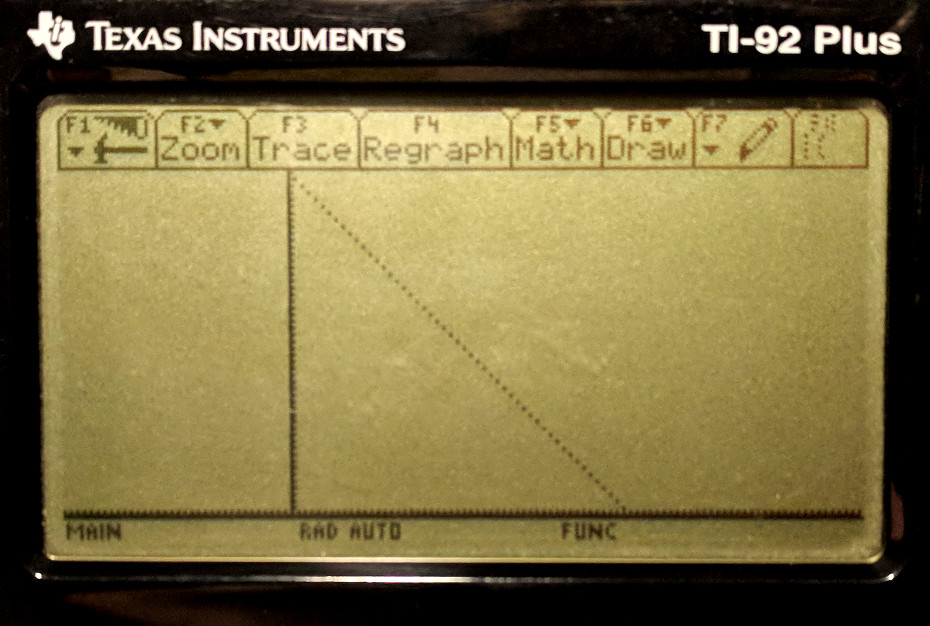
\includegraphics[width=\columnwidth]{not.jpg}
\caption{\label{fig-not-graph} graph of {\tt 255.0f - x} (the bitwise complement of {\tt x}).
{\small Plot created using a TI-92 Plus graphing calculator.}}
\end{figure}

% TODO: Did you mean to include fu8_mod here or above? -tom

For the division and modulus operations, fluint8 diverges from the
normal behavior of integer instructions when the denominator is zero.
A typical processor triggers a fault upon integer division by zero,
but IEEE 754 instead returns one of the special values {\it Infinity},
{\it -Infinity} (or {\it NaN}) and continues calculating. After this
point, fluint8 may produce nonsense results. However, this is strictly
compliant with the C and C++ standard, for which integer division by
zero is formally undefined behavior.\footnote{``If the second operand of / or \% is zero the behavior is undefined.'' --- C++03 5.6.4}

\subsection{Bitwise Operations}

Things really get interesting when we begin to look at bitwise operations, which aren't standard operations on floating point numbers\footnote{Though they seem well-defined; maybe a language-designer oversight?}.

Let's begin with bitwise negation ({\tt \textasciitilde}).
This one is relatively easy to explain -- an unsigned 8-bit integer plus its bitwise complement is always 255, which makes negation as easy as subtraction (Figure~\ref{fig-not-graph}):

{\tt
float fu8\_not(float a) \{ \\
$\phantom{XX}$return 255.0f - a; \\
\}
}

\begin{figure}[tb!]
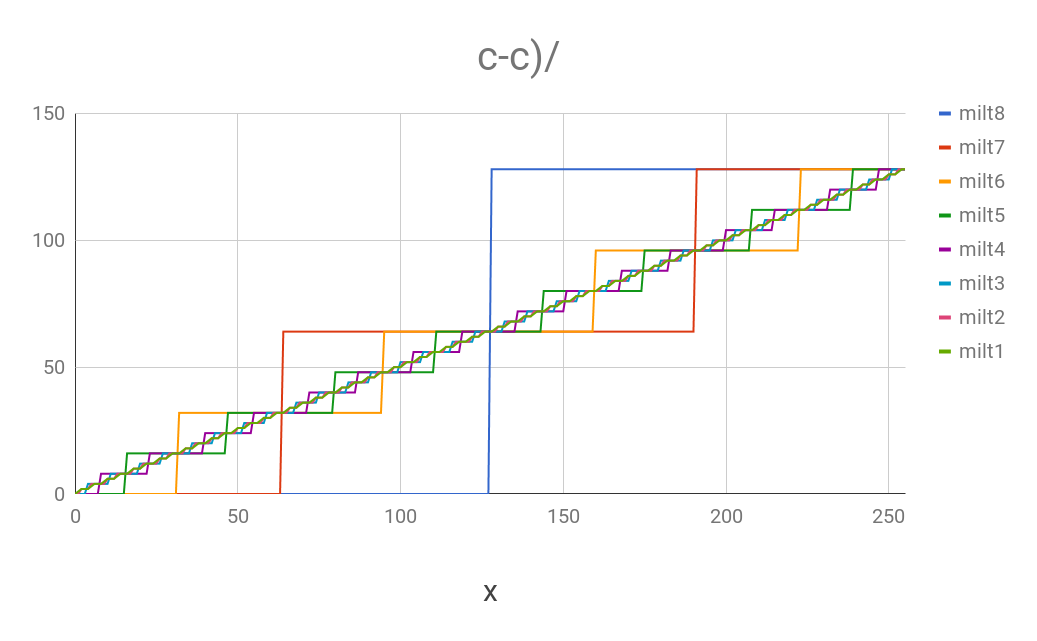
\includegraphics[width=\columnwidth]{milt.png}
\caption{\label{fig-milt-graph}
The value of {\tt a + 1.0f + c-c)/ 2.0f} for {\tt c} ranging from {\tt 2147483648.0f} (milt8) to {\tt 16777216.0f} (milt1).
{\small Plot created in Google Sheets.}
}\end{figure}

Things get a bit more interesting when computing bitwise and ({\tt \&}):

{\tt
float fu8\_and(float a, float b) \{ \\
$\phantom{XX}$float ax, bx, x = 0.0f; \\
$\phantom{XX}$for (float c = 2147483648.0f;\\
$\phantom{XXXXXX}$ c != 8388608.0f; c *= 0.5f) \{ \\
$\phantom{XXXX}$a -= ax = (a + 1.0f + c-c)/ 2.0f; \\
$\phantom{XXXX}$b -= bx = (b + 1.0f + c-c)/ 2.0f; \\
$\phantom{XXXX}$x = 0.5f * x + ax * bx; \\
$\phantom{XX}$\} \\
$\phantom{XX}$return x; \\
\}
}

Note that though this is presented as a loop, the loop has constant bounds and could be unrolled by a compiler into eight repetitions of the same code.

This code peels apart {\tt a} and {\tt b} bit-by-bit using a similar trick to the floating point modulus idea we explained earlier.
In this case, however, we've formatted the code so it has a little waving guy in it, who we will call Milt:

\begin{center}
\huge
{\tt c-c)/}
\end{center}



Though it looks like Milt is just hanging out, minding its own business, and not changing the value of the expression,
Milt is in fact doing something surprisingly nonlinear (Figure~\ref{fig-milt-graph}).



So when Milt's eyes are {\tt 2147483648.0f}, it is extracting twice the value of the MSB of {\tt a},
which in turn is stored in {\tt ax} and subtracted from {\tt a}.
In this way, the code peels off each successive most-significant bit from {\tt a} and {\tt b} and accumulates their product into the final result.

This leaves only the mystery of why {\tt x} is being divided by two each loop iteration.
But this isn't a mystery at all.
Consider computing {\tt 171 \& 226}.
Notice that on the first iteration, the product {\tt 128.0f * 128.0f} would be added to {\tt x};
the multiplications by a factor of {\tt 0.5f} on each subsequent iteration simply -- in aggregate -- bring it to the correct result of {\tt 128.0f}.

{ \tt
\begin{tabular}{r|r|r|r|r|r}
\multicolumn{1}{c|}{a} &
\multicolumn{1}{c|}{b} &
\multicolumn{1}{c|}{ax} &
\multicolumn{1}{c|}{bx} &
\multicolumn{1}{c|}{x} &
\multicolumn{1}{c}{c} \\\hline
171&226& & & & \\
43&98&128&128&16384&2147483648\\
43&34&0&64&8192&1073741824\\
11&2&32&32&5120&536870912\\
11&2&0&0&2560&268435456\\
3&2&8&0&1280&134217728\\
3&2&0&0&640&67108864\\
1&0&2&2&324&33554432\\
0&0&1&0&162&16777216\\

\end{tabular}
}


\section{Optimization}

The previous routine computes a bitwise function a single bit at a
time. While clean and logically motivated, it seems possible to
improve bandwidth by processing multiple bits at once. As a
proof-of-concept, the following routine computes the exclusive-or
function (\verb+^+) for two {\tt fluint}s in the range $0$-$3$.

{ \tt
float fu8\_xor2bit(float a, float b) \{ \\
\phantom{XX}return truncf( \\
\phantom{XXXX}fmod(((a * -1.89269124e+30f) + \\
\phantom{XXXXXXXXXX}(b * -1.09500709e+35f)) * \\
\phantom{XXXXXXXXXXXX}-1.14474456e-18f, \\
\phantom{XXXXXXXXXX}4.77664232f)); \\
\}
}

\begin{figure}[tb!]
\begin{center}
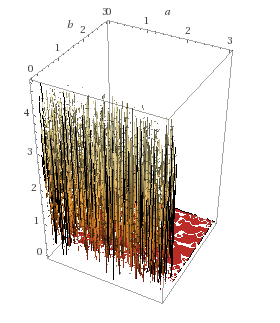
\includegraphics[width=0.6\columnwidth]{xor2bitcube}
\end{center}
\caption{
  3D graph of
  $((a \times -1.89269124 \!\!\times\!\! 10^{30} + (b \times -1.09500709 \!\!\times\!\! 10^{35})) \times -1.14474456 \!\!\times\!\! 10^{-18}) \mod 4.77664232$
  with $a$ and $b$ each ranging from $0$--$3.0$.
%
  {\small Plot created using Wolfram Alpha Computational Knowledge Engine.}} \label{fig:xor2bit}
\end{figure}

The routine works by computing a very noisy function that just happens
to come close to the correct results for all 16 possible inputs. Don't
believe us? Barbecue your eyes of Figure~\ref{fig:xor2bit}. This
routine uses {\tt fmod} and {\tt truncf}, but the same
loss-of-precision tricks from before can likely be used to avoid them.
Four similar expressions can be composed to compute 8-bit exclusive-or,
and/or it may be possible to find expressions that compute more bits
at once.

\section{Not Optimization}

The library should not be used with compiler options such as
\verb+-ffast-math+ (which may assume properties that do not hold of
IEEE754, like commutativity). This often optimizes away the entire
fluint8 code, causing it to misbehave (whoa, not {\em that} fast,
buddy).

\section{Applications}

While direct hardware applications of this technology are currently
theoretical (Section~\ref{sec:future}), there is at least one
compelling application for {\it fluint8} in everyday practice. Many
pieces of software use primarily integer instructions, letting the
floating point unit lie completely dormant for many nanoseconds at a
time. As has been known for decades, while the integer registers and
functional units are occupied, the otherwise idle floating point units
can be used to perform useful tasks. Unfortunately, no useful tasks
were known for floating point instructions. Now, we see that normal
integer operations (such as cryptography) can be simulated with these
instructions and registers. With compiler support, a separate thread
of non-interfering floating point instructions could be emitted, and
arbitrarily interleaved with the integer ones, scheduled only when the
integer unit would likely stall for a data dependency. This technique
is {\em ultrathreading}, since it is one step better than {\em
  hyperthreading}. For example, we hypothesize that during normal web
browsing on a modern x86-64 processor, such code could mine as much as
one Bitcoin per 107 trillion years, with no more than a 1\% loss of
efficiency.

\section{Future Work} \label{sec:future}

Design a processor for which this library is relevant.

\end{document}
